\subsection{Caminos y ciclos}

Consideremos el siguiente grafo:

\begin{figure}
    \centering
    \begin{tikzpicture}
        \GraphInit[vstyle=Normal]
        \SetGraphUnit{2}
        \begin{scope}[rotate=-125]
        \Vertices{circle}{r, u, t, q, p}
        \end{scope}
        \SO[unit=2](q){s}
        \Edges(p, q, t, u, r, p, s, q, r, t, p, s, u, t, s, r)
    \end{tikzpicture}
\end{figure}

\begin{prob}
    De este grafo se desprenden dos problemas:
    \begin{enumerate}
        \item[a)] El Dr. C quiere visitar cada lugar \textit{sólo una vez} y volver al punto de partida.
        \item[b)] El Dr. D quiere recorrer cada ruta sólo una vez (en cualquier sentido). Volver al inicio no es obligatorio.
    \end{enumerate}
\end{prob}

\begin{proof}[Solución al problema]
    Proponemos para ambos problemas las siguientes soluciones:
    \begin{enumerate}
        \item[a)] El Dr. C puede visitar los vértices
        
        \[
        \{ p, q, t, u, r, s, p \}
        \]
        
        y esta solución no es única.
        
        \item[b)] Este problema es más difícil. Llamemos $x$ al punto de partida e $y$ al de llegada, y supongamos que $x \neq y$. Ahora, el Dr. C utiliza un lado cuando parte de $x$, y cada vez que regresa y sale de $x$ ha de hacerlo por lados nuevos. En este sentido, utiliza un número impar de lados en $x$, por lo que $x$ debe ser un vértice impar. De manera similar, $y$ ha de ser impar, ya que utiliza dos lados cada vez que pasa por $y$ y uno último para terminar su recorrido. El resto de los vértices debe ser par, ya que cada vez que se llega al vértice también hay que partir de eĺ.
        
        Entonces, para este ejercicio en particular, tenemos los siguientes grados:
        
        \begin{center}
            \begin{tabular}{cccccc}
                $p$ & $q$ & $r$ & $s$ & $t$ & $u$ \\
                4 & 4 & 5 & 5 & 5 & 3
            \end{tabular}
        \end{center}
        
        Vemos que hay demasiados vértices impares, y en consecuencia no hay ruta para el Dr. D. Si consideramos $x = y$, la situación es incluso peor, pues tendríamos que exigir que todos los vértices sean pares.
    \end{enumerate}
\end{proof}

\begin{defn}
    Dado el grafo $G=(V, L)$, una lista de vértices $v_1, v_2, \dots, v_n$ es un \ul{paseo} si $v_iv_{i+1} \in L$ para $1 \leq i \leq n+1$. Diremos que el paseo es un \ul{camino} si además $v_i \neq v_j$, $\forall i \neq j$. Un \ul{ciclo} es un paseo en el que $v_i=v_n$ y $V_i \neq v_j$ para todo $ij \notin \{1, n\}$.
\end{defn}

\begin{defn}
    Un \ul{ciclo hamiltoniano} sobre un grafo es un ciclo que recorre todos los vértices.
\end{defn}

\begin{defn}
    Un \ul{paseo euleriano} sobre un grafo es un paseo tal que utiliza cada lado exactamente una vez.
\end{defn}

\begin{notn}
    Dados $x, y \in V$, diremos que \textbf{hay un camino} de $x$ a $y$ si existen $v_1, \dots, v_n$ que forman un camino en $G$ tales que $v_1 = x$ y $v_n = y$.
    
    Sintetizamos por decir que \textbf{$x$ está conectado a $y$} es una relación $x \con y$. Esta es una relación de equivalencia.\marginfootnote{Es una relación de equivalencia ya que:
    
    \begin{itemize}
        \item Es reflexiva, pues existen los paseos de un sólo vértice.
        \item Es simétrica, pues para cada camino se puede formar un camino al revés:
        
        \[
        x, v_1, \dots v_n, y \iff y, v_n, \dots, v_1, x
        \]
        
        \item Es transitiva pues si $x \con y$ e $y \con z$, entonces
        
        \begin{gather*}
            x, v_1, \dots v_n, y \wedge y, v'_1, \dots v'_n, z \\
            \implies x, v_1, \dots v_n, y, v'_1, \dots v'_n, z \\
            \iff x \con y
        \end{gather*}
    \end{itemize}}
\end{notn}

\begin{pre}
    Ahora, con esta relación de equivalencia establecida, vale la pena preguntarnos, ¿cómo serán las clases de equivalencia?: Pues serán las componentes del grafo, donde cada uno es un subgrafo. Definimos $G_i=(V_i,L_i)$ a la clase de $v_i$.
\end{pre}

\begin{defn}
    Diremos que un grafo es \ul{conexo} si solo tiene una componente.
\end{defn}

\begin{figure}
    \begin{subfigure}[b]{0.5\textwidth}
    \centering
        \begin{tikzpicture}
            \SetGraphUnit{2}
            \Vertices{circle}{a,b,c,d}
            \Edges(a,b)
            \Edges(c,d)
        \end{tikzpicture}
        \caption{Grafo no conexo}
    \end{subfigure}
    \hfill
    \begin{subfigure}[b]{0.5\textwidth}
    \centering
        \begin{tikzpicture}
            \SetGraphUnit{2}
            \Vertices{circle}{a,b,c,d,e,f,g,h}
            \Edges(a,d,g,b,e,h,c,f,a)
        \end{tikzpicture}
        \caption{Grafo conexo}
    \end{subfigure}
\end{figure}

\subsection{Árboles}

\begin{defn}
    Un \ul{árbol} es un grafo $G=(V,L)$ que cumple:
    
    \begin{enumerate}
        \item[T1] $T$ está conectado.
        \item[T2] No hay ciclos en $T$.
    \end{enumerate}
\end{defn}

Un árbol tiene las siguientes características:

\begin{teo}
    Si $T=(V,L)$ es un árbol con almenos dos vértices, entonces
    
    \begin{enumerate}
        \item[T3] Para todo par $x, y$ hay un único camino en $T$ desde $x$ a $y$.
        \item[T4] El grafo obtenido de $T$ al remover cualquier lado tiene dos componentes, de las cuales cada una es un árbol.
        \item[T5] $|L| = |V|-1$.
    \end{enumerate}
\end{teo}

\begin{proof}
    \begin{enumerate}
        \item[T3] Como $T$ está conectado, entonces hay un camino de $x$ a $y$, luego este camino es
        
        \[
        x, v_1, \dots, v_{r-1}, y
        \]
        
        Supongamos que existe un camino distinto de $x$ a $y$
        
        \[
        x, u_1, \dots, u_{s-1}, y
        \]
        
        donde no necesariamente $r=s$, con $r, s \in \N$.
        
        \begin{figure}
            \centering
            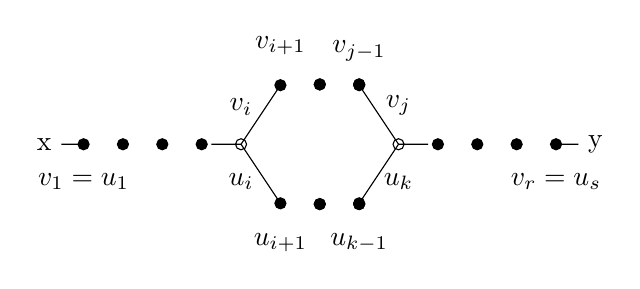
\begin{tikzpicture}[
                level 1/.style = {level distance = 0.5cm},
                level 2/.style = {level distance = 0.5cm}
                ]
                \node at (0,0) {x} [grow = right]
                child {[fill] circle (2pt)};
                \draw (0.5, 0) node[below=7pt] {$v_1 = u_1$};
    	        \filldraw (1,0) circle (2pt);
    	        \filldraw (1.5,0) circle (2pt);
    	        \filldraw (2,0) circle (2pt);
    	        \node at (2,0) {} [grow = right]
    	        child {{[fill] circle (2pt)}
    	        child {[fill] circle (2pt)}
    	        child {[fill] circle (2pt)}};
    	        \draw (2.5, 0) node[above=7pt] {$v_i$};
    	        \draw (2.5, 0) node[below=7pt] {$u_i$};
    	        \draw (3, 0.76) node[above=7pt] {$v_{i+1}$};
    	        \draw (3, -0.76) node[below=7pt] {$u_{i+1}$};
    	        \filldraw (3.5,0.76) circle (2pt);
    	        \filldraw (3.5,-0.76) circle (2pt);
    	        \filldraw (4,0.76) circle (2pt);
    	        \filldraw (4,-0.76) circle (2pt);
    	        \node at (5,0) {} [grow = left]
    	        child {{[fill] circle (2pt)}
    	        child {[fill] circle (2pt)}
    	        child {[fill] circle (2pt)}};
    	        \draw (4.5, 0) node[above=7pt] {$v_j$};
    	        \draw (4.5, 0) node[below=7pt] {$u_k$};
    	        \draw (4, 0.69) node[above=7pt] {$v_{j-1}$};
    	        \draw (4, -0.76) node[below=7pt] {$u_{k-1}$};
    	        \filldraw (3.5,0.76) circle (2pt);
    	        \filldraw (3.5,-0.76) circle (2pt);
    	        \filldraw (4,0.76) circle (2pt);
    	        \filldraw (4,-0.76) circle (2pt);
    	        \node at (7,0) {y} [grow = left]
                child {[fill] circle (2pt)};
                \draw (6.5, 0) node[below=7pt] {$v_r = u_s$};
    	        \filldraw (6,0) circle (2pt);
    	        \filldraw (5.5,0) circle (2pt);
    	        \filldraw (5,0) circle (2pt);
            \end{tikzpicture}
            \caption{Representación del ciclo, y de la eventual contradicción.}
            \label{fig:falsot}
        \end{figure}
        
        Entonces sea $i$ el menor subíndice para el cual $u_{i+1} \neq v_{i+1}$. Como ambos caminos terminan en $y$, podemos definir un $j$ tal que es el menor subíndice para el cual
        
        \[
        j > i \wedge v_{j} = u_{k} \quad \text{para algún} k
        \]
        
        Luego, $v_i, v_{i+1}, \dots, v_j, u_{k-1}, u_{k-2}, \dots, u_{i+1}, v_i$ es un ciclo en $T$, contrario a la definición de árbol.
        
        \item[T4] Supongamos que $uv$ es un lado de $T$, y sea $S = (V, E')$ un grafo tal que $E' = E \backslash uv$. Sea ahora $V_1$ un subconjunto de $V$ tal que existe un camino único desde $x$ a $v$ tal que $x \in V$ y dicho camino pasa por $u$. Claramente, todos estos caminos deben terminar en el lado $uv$, ya que de lo contrario tendríamos ciclos en $T$, cosa que es imposible.
        
        Sea ahora $V_2 = V_1^c$. Cada vértice en $V_1$ tiene un camino a $u$ contenido en $S$, y cada vértice en $V_2$ tiene un camino a $v$ contenido en $S$, pero no hay camino de $v$ a $u$ en $S$. Se sigue que $V_1$ y $V_2$ son los conjuntos de vértices de dos componentes de $S$. Cada componente por definición está conectada, y no tienen ciclos, ya que no hay ciclos en $T$. Por lo tanto, dichas componentes son árboles.
        
        \item[T5] Procedamos con un argumento inductivo: En primer lugar, esto se cumple para $|V| = 1$, ya que el único árbol que se puede construir con un único vértice no tiene lados.
        
        Supongamos que la propiedad es cierta para $|V| \leq k$, y sea $T$ un árbol con $|V| = k+1$, y sea $uv$ cualquier lado de $T$. Si $T_1 = (V_1, E_1)$ y $T_2 = (V_2, E_2)$ son los árboles obtenidos de quitar el lado $uv$ de $T$, tenemos que
        
        \[
        |V_1| + |V_2| = |V| \quad |L_1| + |L_2| = |L| - 1
        \]
        
        \noindent utilizando ahora la hipótesis inductiva, tenemos
        
        \[
        |L| = |L_1| + |L_2| + 1 = |V_1| - 1 + |V_2| - 1 + 1 = |V_1| + |V_2| - 1 = |V| - 1
        \]
        
        \noindent de esta forma, $|L| = |V| - 1$, y queda demostrado para todos los enteros positivos $k$.
    \end{enumerate}
\end{proof}